\documentclass[tikz, border=15pt]{standalone}
\usepackage{amsmath}
\usetikzlibrary{calc, patterns, decorations.pathreplacing}

% Define the exact color from your prompt
\definecolor{mygreen}{HTML}{00d1b2}

\begin{document}
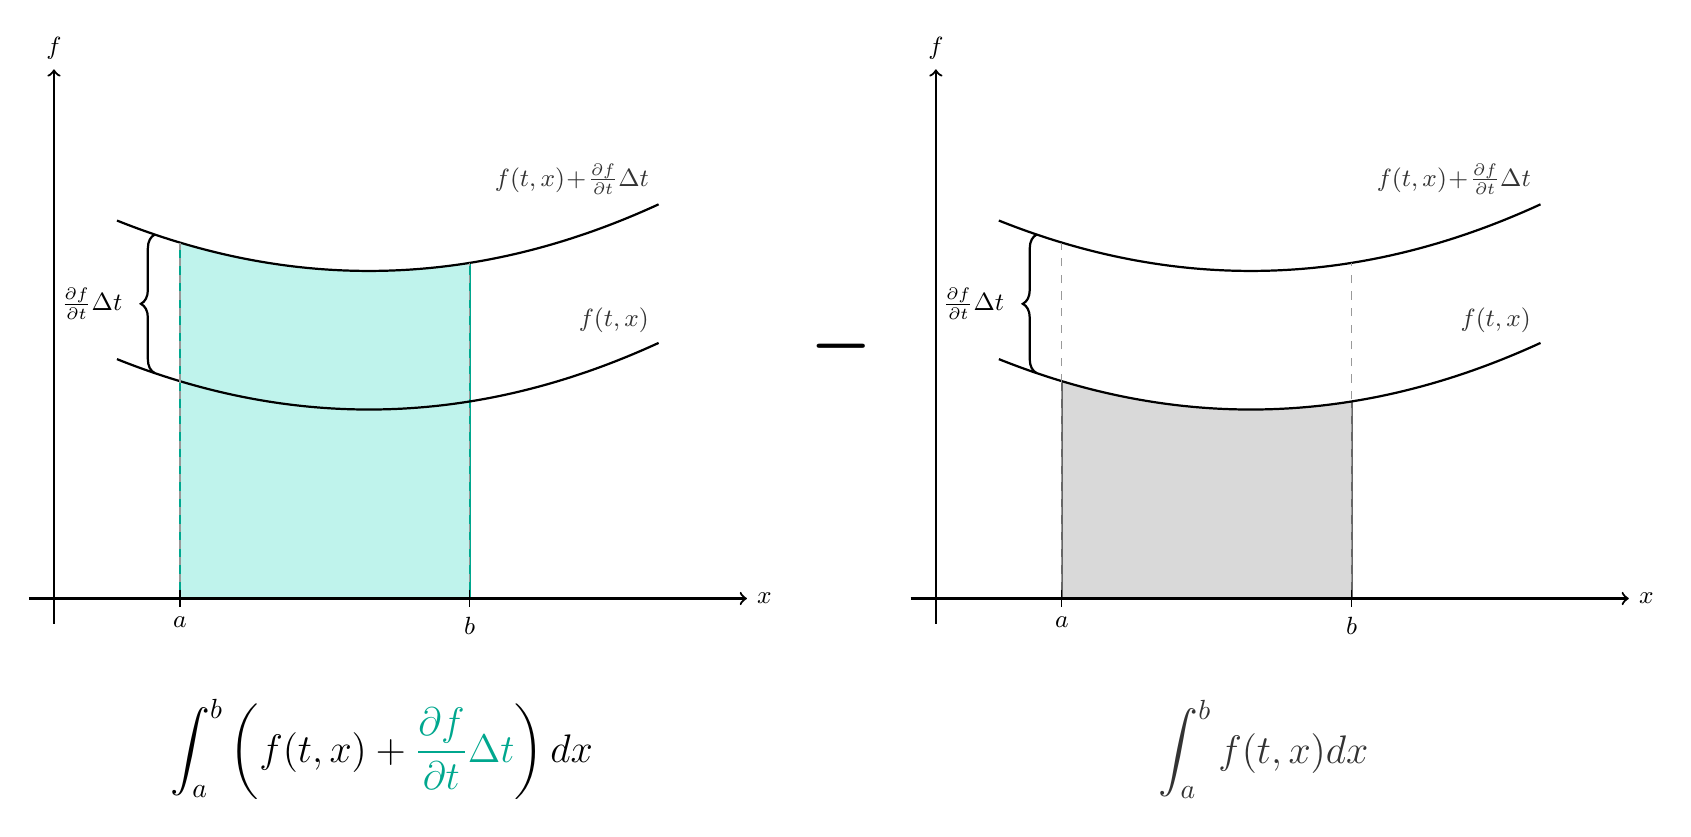
\begin{tikzpicture}[
    scale=1.6, % Scale adjusted for a 1x2 layout
    every node/.style={font=\small},
    label box/.style={align=center}
]

    % --- 1. DEFINE SHARED FUNCTIONS AND VARIABLES ---
    % Bottom curve: f(t, x)
    \pgfmathdeclarefunction{funcF}{1}{\pgfmathparse{0.1*(#1-2.5)^2 + 1.5}}
    % Top curve: f(t, x) + df/dt * dt
    \pgfmathdeclarefunction{funcFdt}{1}{\pgfmathparse{0.1*(#1-2.5)^2 + 2.6}}

    \def\a{1.0} 
    \def\b{3.3} 
    
    \def\shiftY{1.1}
    \def\xLeft{0.8}

    % \W is the horizontal step between the two diagrams
    \def\W{7.0} 

    % --- 2. MACRO TO DRAW THE BASE SCENE EVERY TIME ---
    \def\drawBase{
        % Axes
        \draw[->, thick] (-0.2,0) -- (5.5,0) node[right] {$x$};
        \draw[->, thick] (0,-0.2) -- (0,4.2) node[above] {$f$};

        % Curves
        \draw[thick] plot[domain=0.5:4.8, samples=100] (\x, {funcF(\x)});
        \draw[thick] plot[domain=0.5:4.8, samples=100] (\x, {funcFdt(\x)});

        % Curve Labels
        \node[above left, text=black!80] at (4.8, {funcF(4.8)}) {$f(t,x)$};
        \node[above left, text=black!80] at (4.8, {funcFdt(4.8)}) {$f(t,x) \!+\! \frac{\partial f}{\partial t}\Delta t$};

        % Dashed Boundary Lines (Only at a and b)
        \draw[dashed, thin, gray!80] (\a,0) -- (\a, {funcFdt(\a)});
        \draw[dashed, thin, gray!80] (\b,0) -- (\b, {funcFdt(\b)});

        % X-Axis Marks
        \draw (\a, 2pt) -- (\a, -2pt) node[below] {$a$};
        \draw (\b, 2pt) -- (\b, -2pt) node[below] {$b$};

        % Vertical Brace for the shift df/dt * dt
        \pgfmathsetmacro{\fxL}{funcF(\xLeft)}
        \pgfmathsetmacro{\fxdtL}{funcFdt(\xLeft)}
        \draw[decorate, decoration={brace, amplitude=5pt}, thick] 
            (\xLeft, \fxL) -- (\xLeft, \fxdtL) 
            node[midway, left=8pt] {$\frac{\partial f}{\partial t}\Delta t$};
    }


    % ==========================================
    % PANEL 1: (The Expanded Shifted Area)
    % ==========================================
    \begin{scope}[shift={(0,0)}]
        % Fill Area
        \fill[mygreen, fill opacity=0.25] (\a,0) -- plot[domain=\a:\b, samples=100] (\x, {funcFdt(\x)}) -- (\b,0) -- cycle;
        \draw[mygreen!80!black, thick] (\a,0) -- (\a, {funcFdt(\a)});
        \draw[mygreen!80!black, thick] (\b,0) -- (\b, {funcFdt(\b)});
        
        \drawBase % Overlay base scene
        
        % Label below (highlighting the partial derivative term)
        \node[label box] at (2.6, -1.2) 
            {\Large $\displaystyle \int_a^b \left(f(t,x) + {\color{mygreen!80!black}\frac{\partial f}{\partial t}\Delta t}\right) dx$};
    \end{scope}

    % Operator - (Centered exactly between the graphs)
    \node at (6.25, 2.0) {\Huge $\boldsymbol{-}$};

    % ==========================================
    % PANEL 2: (The Original Base Area)
    % ==========================================
    \begin{scope}[shift={(\W,0)}]
        % Fill Area
        \fill[black, fill opacity=0.15] (\a,0) -- plot[domain=\a:\b, samples=100] (\x, {funcF(\x)}) -- (\b,0) -- cycle;
        \draw[black!60, thick] (\a,0) -- (\a, {funcF(\a)});
        \draw[black!60, thick] (\b,0) -- (\b, {funcF(\b)});
        
        \drawBase % Overlay base scene
        
        % Label below
        \node[label box, text=black!80] at (2.6, -1.2) 
            {\Large $\displaystyle \int_a^b f(t,x) dx$};
    \end{scope}

\end{tikzpicture}
\end{document}